\documentclass[tikz,border=5]{standalone}
\usetikzlibrary{decorations.pathmorphing}
\usepackage[detect-all]{siunitx}

\tikzset{
   ragged border/.style={ decoration={random steps, segment length=1mm, amplitude=0.5mm},
           decorate,
   }
}

\begin{document}
  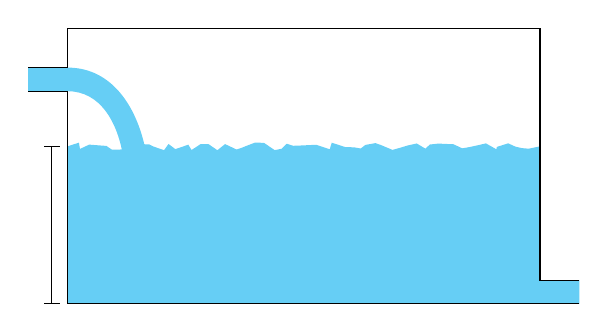
\begin{tikzpicture}
  \fill[cyan!60]
        decorate[ragged border]{
        (0,2) -- (6,2)
        }
        -- (6,0.3) -- (6.5,0.3) -- (6.5,0.0) -- (6,0.0) --(6,0) -- (0,0) -- cycle;
  \fill[cyan!60] (-0.5,2.7) -- (0,2.7) to[in=100,out=0](0.7,1.9)-- (1.0,1.9)
                  to[out=100,in=0] (0,3) -- (-0.5,3) -- cycle;
  \draw (-0.5,2.7) -- (0,2.7) -- (0,0) -- (6,0) -- (6,0.0) -- (6.5,0.0);
  \draw (-0.5,3) -- (0,3) -- (0,3.5) -- (6,3.5) -- (6,0.3) -- (6.5,0.3);
  \draw[|-|] (-0.2,0) --
        node[fill=white,font=\footnotesize,inner ysep=2pt,inner
                xsep=0, anchor=east]{}(-0.2,2);
  %\draw[stealth-] (-0.5,2.75) -- (-1,2.75)
  %          node[anchor=east,font=\footnotesize,align=right]{};
  %\draw[-stealth] (6.5,0.15) -- (7.2,0.15)
  %          node[anchor=west,font=\footnotesize]{};
  \node[anchor=north,font=\footnotesize] at (3,3) {};
  \node[anchor=north,font=\footnotesize] at (3,2) {};
  \node[anchor=north,font=\footnotesize] at (3,1) {};
\end{tikzpicture}%
\end{document}